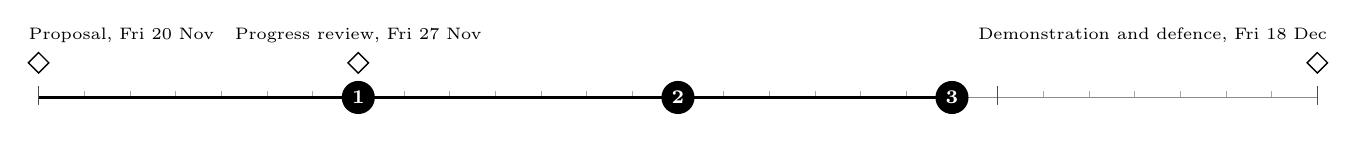
\begin{tikzpicture}[x=1mm,y=1mm,
  ev/.style={font=\figfont\fontsize{6.4}{7.2}\selectfont,inner sep=0pt},
  ms/.style={anchor=north west,text width=50mm,align=left,inner sep=0pt,font=\small,
    execute at begin node={\hyphenpenalty=10000\exhyphenpenalty=10000\raggedright}}]
\def\ox{1.3}\def\dd{5.8}
% the whole period, its days and weeks, then the working period in heavy black
\draw[line width=0.35pt,black!45] (\ox,0) -- ({\ox+\dd*28},0);
\foreach \g in {0,...,28} {\draw[line width=0.25pt,black!35] ({\ox+\dd*\g},0) -- ({\ox+\dd*\g},0.8);}
\foreach \g in {0,7,14,21,28} {\draw[line width=0.4pt,black!70] ({\ox+\dd*\g},-0.9) -- ({\ox+\dd*\g},1.5);}
\draw[line width=1.1pt] (\ox,0) -- ({\ox+\dd*20},0);
% course dates above the axis
\foreach \g/\t/\a/\dx in {0/{Proposal, Fri 20 Nov}/base west/-1.3,7/{Progress review, Fri 27 Nov}/base/0,28/{Demonstration and defence, Fri 18 Dec}/base east/1.3} {
  \draw[line width=0.5pt,fill=white] ({\ox+\dd*\g},4.4) +(0,1.3) -- +(1.3,0) -- +(0,-1.3) -- +(-1.3,0) -- cycle;
  \node[ev,anchor=\a] at ({\ox+\dd*\g+\dx},7.4) {\t};}
% milestones on the axis
\foreach \g/\n/\cx in {7/1/0,14/2/57.5,20/3/115} {
  \fill ({\ox+\dd*\g},0) circle (2.1mm);
  \node[text=white,font=\figfont\bfseries\fontsize{7.4}{7.4}\selectfont] at ({\ox+\dd*\g},0) {\n};}
\end{tikzpicture}
